%%%%%%%%%%%%
%
% $Autor: Wings $
% $Datum: 2019-03-05 08:03:15Z $
% $Pfad: SetUp.tex $
% $Version: 4250 $
% !TeX spellcheck = en_GB/de_DE
% !TeX encoding = utf8
% !TeX root = manual 
% !TeX TXS-program:bibliography = txs:///biber
%
%%%%%%%%%%%%

\chapter{Setup}

This section guides you through preparing your environment and project files before running the Hurricane Intensity Prediction System. Please follow each step carefully.

\section*{Project Folder Structure}

Your main project folder should be named \texttt{hurricane\_predictor\_ready} and contain the following files and folders:

\begin{verbatim}
	hurricane_predictor_ready/
	|
	+-- app.py
	+-- developer.py
	+-- models_train.py
	+-- utils.py
	+-- requirements.txt
	+-- models/         # Folder for storing trained model files
	+-- data/           # Folder for datasets
\end{verbatim}

\section*{Initial Steps}

\begin{enumerate}
	\item \textbf{Clone or Download the Repository:} \\
	Download the project from the official source or clone it using:
	\begin{verbatim}
		git clone https://github.com/yourusername/hurricane_predictor_ready.git
	\end{verbatim}
	
	\item \textbf{Create and Activate a Virtual Environment:} \\
	Open your terminal or command prompt, navigate to the project folder, and run:
	\begin{verbatim}
		python3 -m venv venv
	\end{verbatim}
	Activate the environment:
	\begin{itemize}
		\item On Linux/Mac:
		\begin{verbatim}
			source venv/bin/activate
		\end{verbatim}
		\item On Windows:
		\begin{verbatim}
			venv\Scripts\activate
		\end{verbatim}
	\end{itemize}
	
	\item \textbf{Install Required Libraries:} \\
	With the virtual environment activated, install dependencies:
	\begin{verbatim}
		pip install -r requirements.txt
	\end{verbatim}
	
	\item \textbf{Check Model Files:} \\
	Ensure the \texttt{models/} folder contains the pre-trained ARIMA and LSTM model files. If not, contact the developer or use \texttt{developer.py} to train and save the models.
	
	\item \textbf{Prepare Your Data:} \\
	Place your hurricane dataset (CSV format) in the \texttt{data/} folder, or have it ready for upload via the app interface. The file should include at least \texttt{datetime} and \texttt{wind\_speed} columns.
	
	\item \textbf{Test the Setup:} \\
	Run the following command:
	\begin{verbatim}
		streamlit run app.py
	\end{verbatim}
	The application should launch in your web browser without errors.
\end{enumerate}

\section*{Setup Workflow Diagram}

\begin{figure}[h]
	\centering
	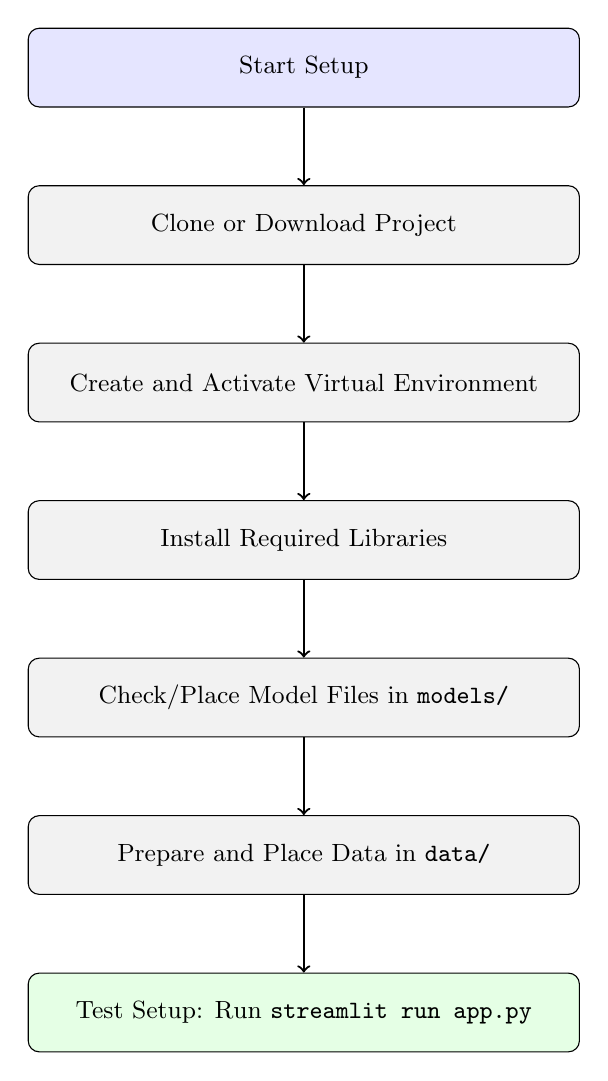
\begin{tikzpicture}[
		node distance=2cm,
		every node/.style={draw, rounded corners, minimum width=7cm, minimum height=1cm, align=left, font=\small}
		]
		\node[fill=blue!10] (start) {Start Setup};
		\node[below of=start, fill=gray!10] (clone) {Clone or Download Project};
		\node[below of=clone, fill=gray!10] (venv) {Create and Activate Virtual Environment};
		\node[below of=venv, fill=gray!10] (install) {Install Required Libraries};
		\node[below of=install, fill=gray!10] (models) {Check/Place Model Files in \texttt{models/}};
		\node[below of=models, fill=gray!10] (data) {Prepare and Place Data in \texttt{data/}};
		\node[below of=data, fill=green!10] (test) {Test Setup: Run \texttt{streamlit run app.py}};
		
		\draw[->, thick] (start) -- (clone);
		\draw[->, thick] (clone) -- (venv);
		\draw[->, thick] (venv) -- (install);
		\draw[->, thick] (install) -- (models);
		\draw[->, thick] (models) -- (data);
		\draw[->, thick] (data) -- (test);
	\end{tikzpicture}
	\caption{Setup Workflow for Hurricane Intensity Prediction System}
\end{figure}

\textbf{Tip:} If you encounter any issues during setup, refer to the \textbf{Troubleshooting} chapter for solutions.


